\documentclass[../sections/subsections/probabilidad_condicional.tex]{subfiles}

% Set the overall layout of the tree
\tikzstyle{level 1}=[level distance=3.5cm, sibling distance=3.5cm]
\tikzstyle{level 2}=[level distance=3.5cm, sibling distance=2cm]

% Define styles for bags and leafs
\tikzstyle{urna} = [text width=4em, text centered]
\tikzstyle{end} = [circle, minimum width=3pt,fill, inner sep=0pt]

% The sloped option gives rotated edge labels. Personally
% I find sloped labels a bit difficult to read. Remove the sloped options
% to get horizontal labels. 
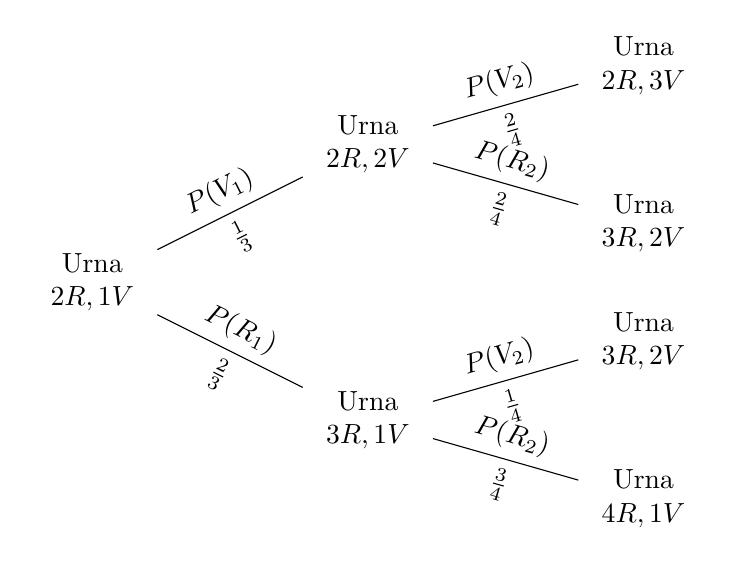
\begin{tikzpicture}[grow=right, sloped]
\node[urna] {Urna $2R, 1V$}
    child {
        node[urna] {Urna $3R, 1V$}        
            child {
                node[urna] {Urna $4R, 1V$}
                edge from parent
                node[above] {$P(R_{2})$}
                node[below]  {$\frac{3}{4}$}
            }
            child {
                node[urna] {Urna $3R, 2V$}
                edge from parent
                node[above] {$P(V_{2})$}
                node[below]  {$\frac{1}{4}$}
            }
            edge from parent 
            node[above] {$P(R_{1})$}
            node[below]  {$\frac{2}{3}$}
    }
    child {
        node[urna] {Urna $2R, 2V$}        
        child {
                node[urna] {Urna $3R, 2V$}
                edge from parent
                node[above] {$P(R_{2})$}
                node[below]  {$\frac{2}{4}$}
            }
            child {
                node[urna] {Urna $2R, 3V$}
                edge from parent
                node[above] {$P(V_{2})$}
                node[below]  {$\frac{2}{4}$}
            }
        edge from parent         
            node[above] {$P(V_{1})$}
            node[below]  {$\frac{1}{3}$}
    };
\end{tikzpicture}